\documentclass[]{article}

\usepackage[margin=2cm]{geometry}
\usepackage{amsmath}
\usepackage{hyperref}
\usepackage{cleveref}
\usepackage{svg}

\definecolor{darkpastelgreen}{rgb}{0.01, 0.75, 0.24}

\title{%
    ELEC 0041: Homework 1\\
    \large Design of a DC busbar
}
\author{Tomasetti Romin}

\begin{document}

\maketitle

\begin{abstract}
    This is the report for the first homework of the course ELEC0041.
    The goal is to optimize a copper busbar such that the current arriving from an input port
    is evenly distributed to 3 output ports.
    \footnote{\url{https://github.com/romintomasetti/elec0041/}}
\end{abstract}

\section{Simulation setup}

In this section, the simulated geometry is briefly described.
A simple mesh convergence analysis is also conducted.
Eventually, orders of magnitude of the simulated fields are verified.

\subsection{Geometry and modeling}

The simulated geometry is shown in~\Cref{figure:geometry}.
This geometry differs from the problem statement in that it takes the symmetry of the problem into account.
An ellipse has been added to balance the current distribution amongst the three output ports.

Note that the simulation will be carried out considering that a 2D approximation is acceptable, i.e.
perfect conductors are assumed for the connectors and 3D effects are neglected.

\begin{figure}[h]
    \centering
    \includesvg[width=0.25\textwidth]{homework-1/report/geometry.svg}
    \caption{Simulated geometry.}
    \label{figure:geometry}
\end{figure}

\subsection{Convergence of the mesh}

In this section, a simple mesh convergence analysis is conducted.
The mesh is driven by 4 parameters, namely the element size on the top and bottom copper plate borders,
on the input and output ports, and on the balancing hole.

The convergence is observed using a globally integrated quantity, namely the losses.
The left and middle output port currents are also monitored.
As can be seen in~\Cref{figure:mesh-convergence}, the quantities are nearly converged at the green cross,
which is a parametrization that has a good percision/computing cost trade-off.

It must be noted that even though the ellipse's center will move vertically and minor and major axes will change,
the mesh parametrization will be kept unchanged for simplicity.

\section{Orders of magnitude}


According to Pouillet's law, the resistance is given by $R = \rho l / A$.
In this case, considering that the length $l$ is the distance between the left-most output port
and the input port, it leads to:
%
\begin{equation}
    R \approx \rho /t \approx 1.72 \cdot 10^{-8} / 2 \cdot 10^{-3} \approx 0.86 \cdot 10^{-5} \Omega,
\end{equation}
%
where $t$ is the thickness of the copper plate and $\rho$ is the annealed copper resistivity
\footnote{The annealed copper resistivity and conductivity can be found in
\url{http://hyperphysics.phy-astr.gsu.edu/hbase/Tables/rstiv.html}.}.
Then, using Ohm's law with one third of the input current, the expected voltage magnitude is
%
\begin{equation}
    V = R I = \cfrac{375}{3} \cdot 0.86 \cdot 10^{-5} = 1.075 \cdot 10^{-3} \ V
\end{equation}
\section{Design optimization}

Explain the choice of design optimization, i.e. why an ellipse.

An ellipse is simple to machine.

\subsection{Brute force optimization}

\subsection{Sensivity near optimal point}

\pagebreak

\section{Supplementary figures}

\begin{figure}[h]
    \centering
    \includesvg[width=\textwidth]{homework-1/test_mesh_convergence.svg}
    \caption{
        Convergence study.
        The mesh is driven by 4 parameters, namely the size of the elements on the top and bottom borders of the copper plate,
        on the input and output parts and on the ellipse.
        Their relative proportions are kept constant.
        The \textcolor{darkpastelgreen}{green cross} represents the chosen mesh parametrization.
    }
    \label{figure:mesh-convergence}
\end{figure}

% Title: v.sym
% Creator: GL2PS 1.4.3, (C) 1999-2020 C. Geuzaine
% For: Gmsh
% CreationDate: Thu Mar 10 10:27:29 2022
\setlength{\unitlength}{0.1403pt}
\begin{picture}(0,0)
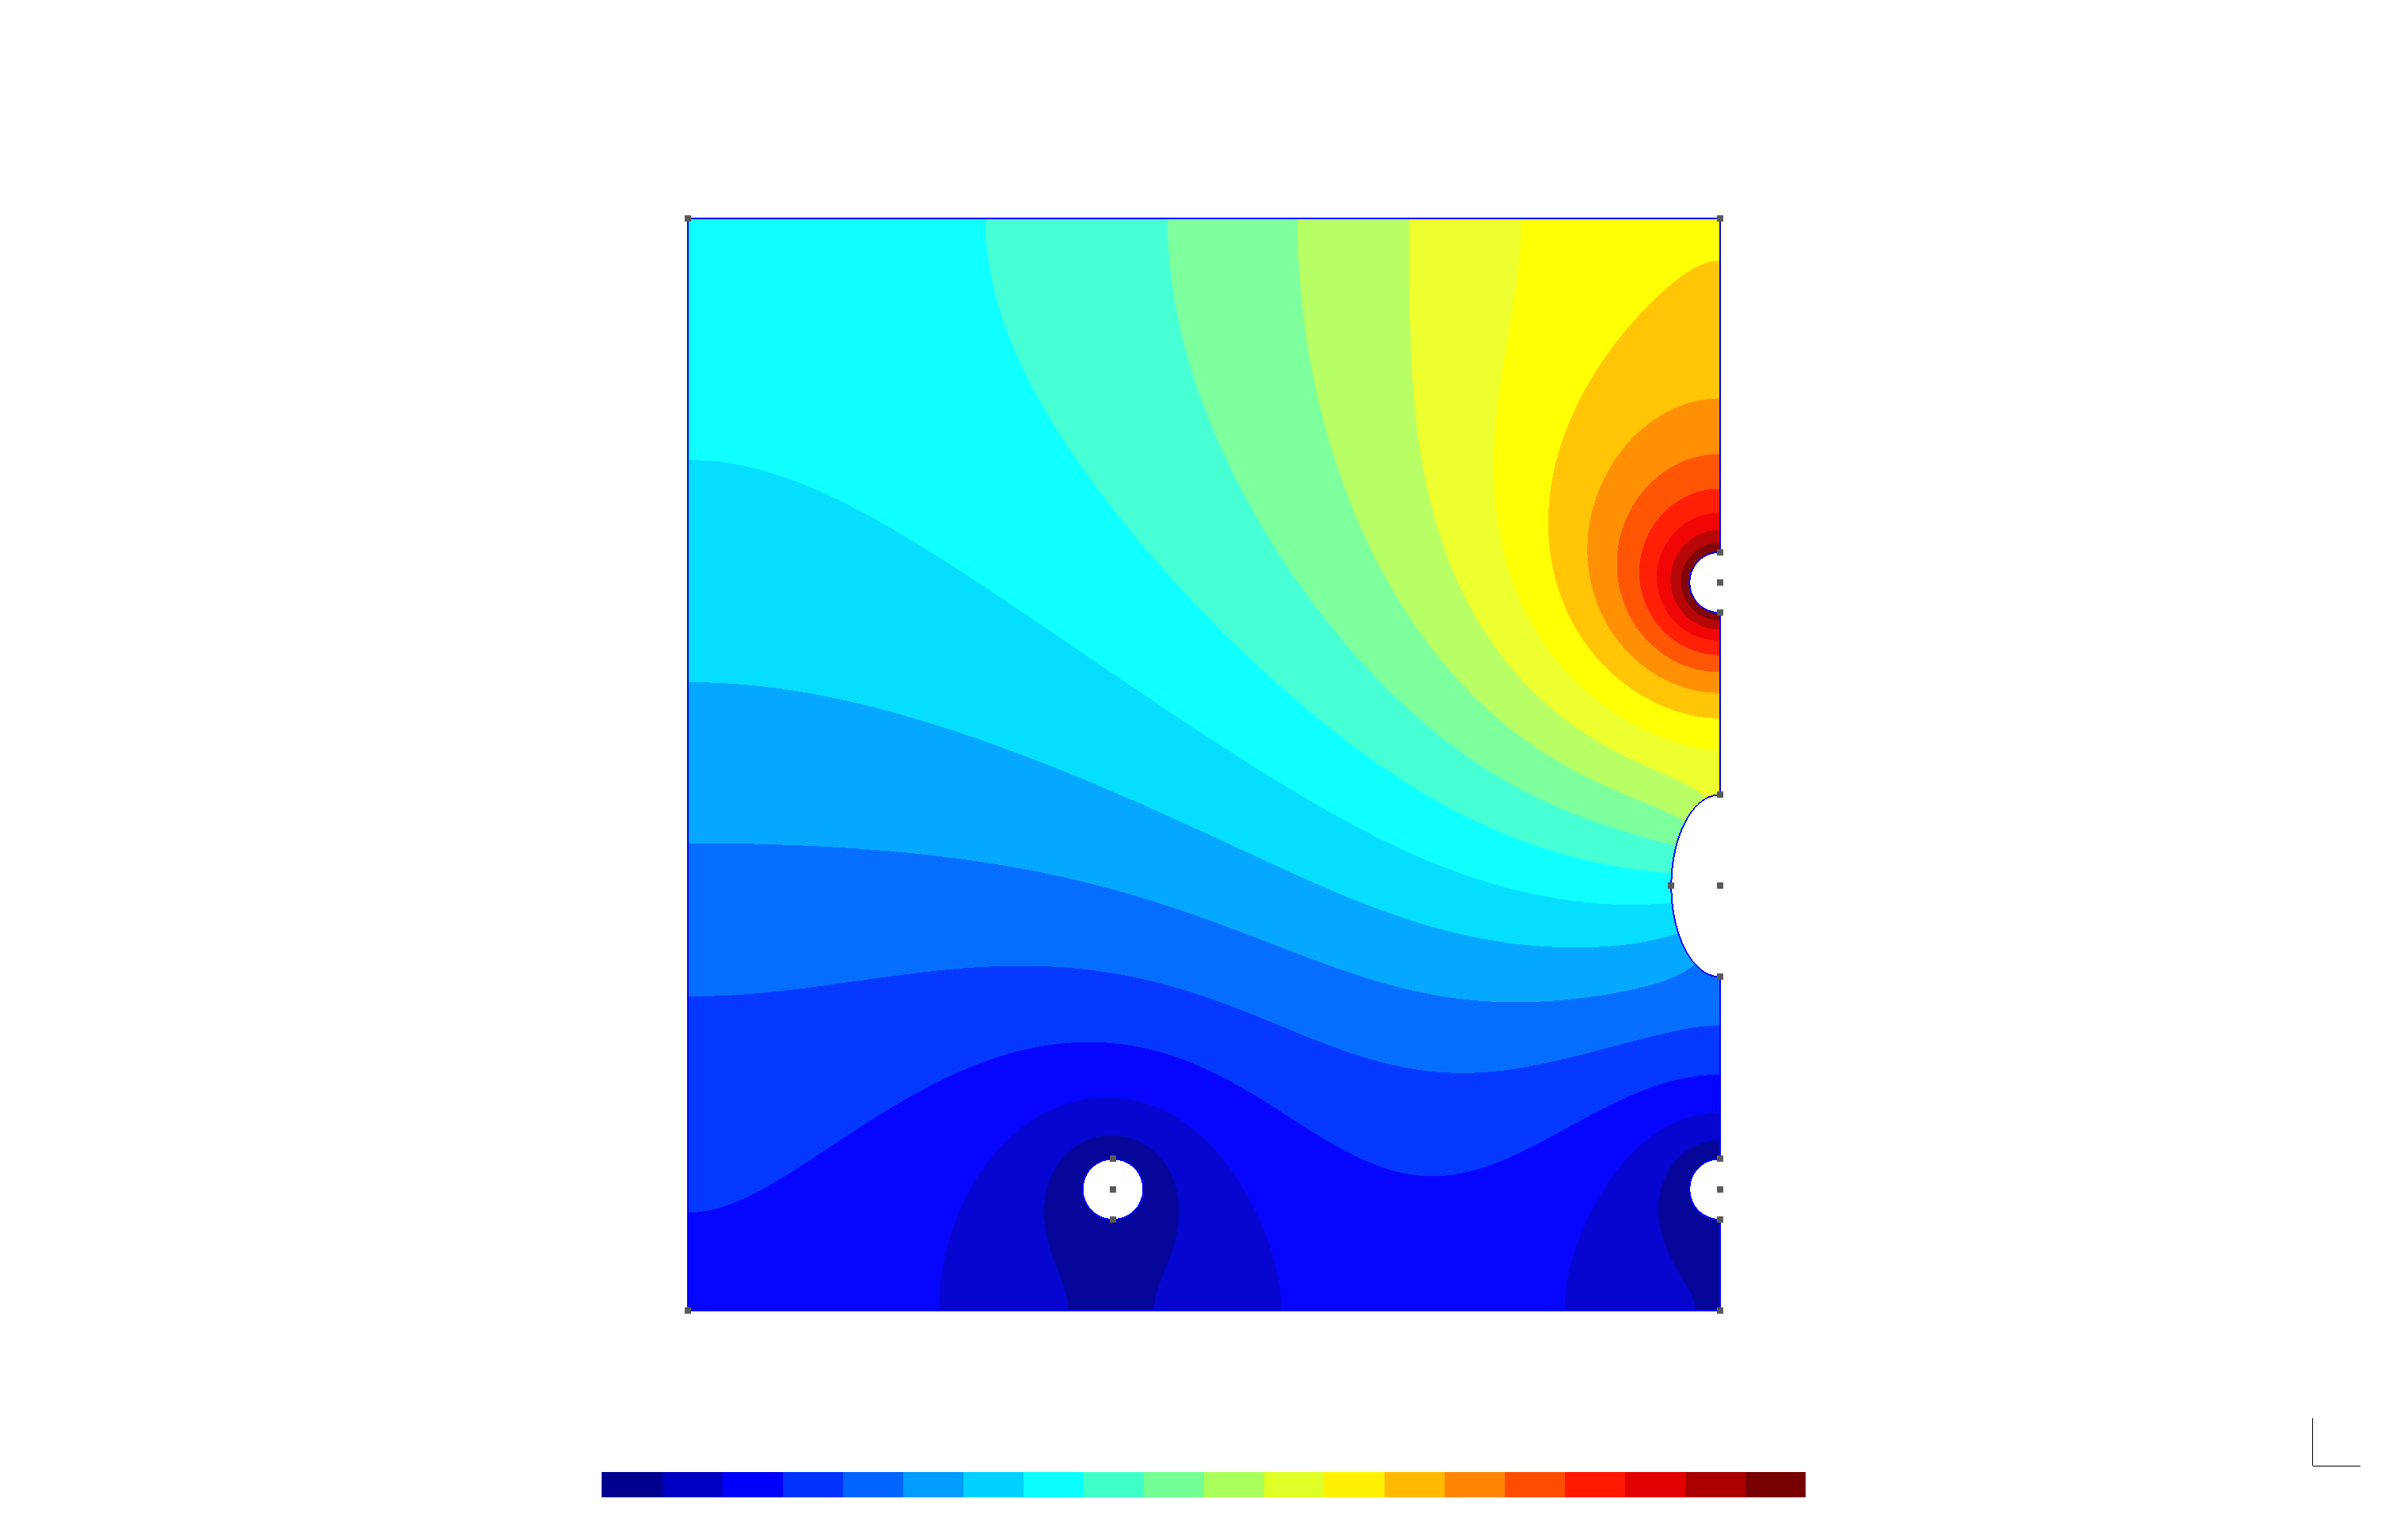
\includegraphics[scale=0.1403]{homework-1/v.sym.png}
\end{picture}%
\begin{picture}(3042,1932)(0,0)
\put(760.5,92){\makebox(0,0)[b]{\textcolor[rgb]{0,0,0}{{0}}}}
\put(1521,92){\makebox(0,0)[b]{\textcolor[rgb]{0,0,0}{{0.00125}}}}
\put(2281.5,92){\makebox(0,0)[b]{\textcolor[rgb]{0,0,0}{{0.0025}}}}
\put(1521,142.4){\makebox(0,0)[b]{\textcolor[rgb]{0,0,0}{{Scalar electric potential [V]}}}}
\put(2988,86){\makebox(0,0)[bl]{\textcolor[rgb]{0,0,0}{{X}}}}
\put(2928,146){\makebox(0,0)[bl]{\textcolor[rgb]{0,0,0}{{Y}}}}
\put(2928,86){\makebox(0,0)[bl]{\textcolor[rgb]{0,0,0}{{Z}}}}
\end{picture}


\end{document}
